\documentclass[10pt,a4paper]{article}

% Portfolio-facing modern résumé with a photo-led identity and extractable text.
\usepackage{iftex}
\ifPDFTeX
  \usepackage[T1]{fontenc}
  \usepackage[utf8]{inputenc}
  \usepackage{lmodern}
  \input{glyphtounicode}
  \pdfgentounicode=1
\else
  \usepackage{fontspec}
  \setmainfont{lmroman10-regular.otf}[
    BoldFont       = lmroman10-bold.otf,
    ItalicFont     = lmroman10-italic.otf,
    BoldItalicFont = lmroman10-bolditalic.otf,
    Ligatures      = NoCommon
  ]
\fi

\usepackage[a4paper,top=0.32in,bottom=0.32in,left=0.34in,right=0.34in]{geometry}
\usepackage{graphicx}
\usepackage{enumitem}
\usepackage[hidelinks]{hyperref}
\usepackage{xcolor}
\usepackage{array}

\definecolor{accent}{HTML}{38E8B5}
\definecolor{accentdark}{HTML}{087F67}
\definecolor{sidebar}{HTML}{F1F3F4}
\definecolor{ink}{HTML}{101416}
\definecolor{muted}{HTML}{4B5563}
\definecolor{rulecolor}{HTML}{1F2937}

\pagestyle{empty}
\setlength{\parindent}{0pt}
\setlength{\parskip}{0pt}
\setlength{\fboxsep}{0pt}
\urlstyle{same}
\color{ink}
\raggedright
\setlist[itemize]{leftmargin=1.05em,itemsep=0.7pt,topsep=1.3pt,parsep=0pt,partopsep=0pt,label=\textbullet}

\newcommand{\mainsection}[1]{%
  \vspace{3pt}{\fontsize{14}{16}\selectfont\bfseries #1}\par
  \vspace{1pt}{\color{rulecolor}\hrule height 0.55pt}\vspace{2pt}
}

\newcommand{\sidesection}[1]{%
  \vspace{6pt}{\large\bfseries #1}\par
  \vspace{1pt}{\color{rulecolor}\hrule height 0.45pt}\vspace{3pt}
}

\newcommand{\project}[3]{%
  \textbf{#1}\hfill{\scriptsize\colorbox{accent}{\hspace{3pt}#2\hspace{3pt}}}\par
  {\small\textit{#3}}\par
}

\newcommand{\skillgroup}[2]{%
  \textbf{#1}\par
  {\small #2}\par\vspace{4pt}
}

\begin{document}
\fontsize{9.2}{10.5}\selectfont

% Header adapted from the supplied photo template.
{\setlength{\fboxsep}{9pt}%
\colorbox{accent}{%
  \begin{minipage}[c][3.45cm][c]{\dimexpr\textwidth-18pt\relax}
    \begin{minipage}[c]{0.22\linewidth}
      \centering
      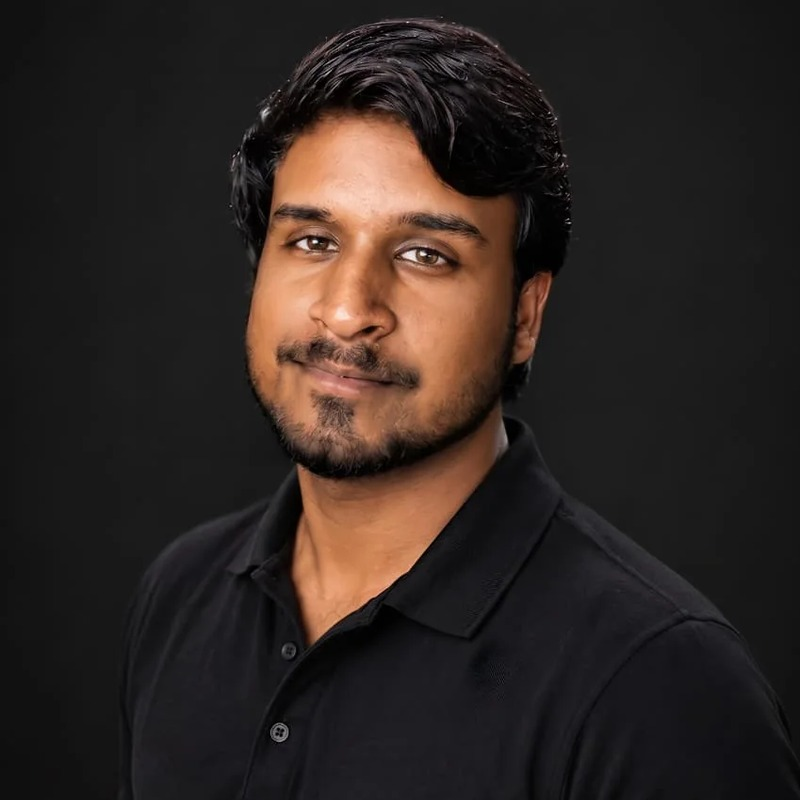
\includegraphics[width=3.05cm,height=3.05cm]{shivansh-goel-headshot.jpg}
    \end{minipage}\hfill
    \begin{minipage}[c]{0.73\linewidth}
      {\fontsize{25}{27}\selectfont\bfseries SHIVANSH GOEL}\par
      \vspace{2pt}
      {\large\bfseries AI Developer \textbar{} Fourth-Year B.Tech Student}\par
      \vspace{7pt}
      {\small
        \href{mailto:shivansh.goela12@gmail.com}{shivansh.goela12@gmail.com}
        \quad\textbar\quad +91 9458569110
        \quad\textbar\quad Delhi, India
      }\par
      \vspace{2pt}
      {\small
        \href{https://github.com/Tech-aficionado}{github.com/Tech-aficionado}
        \quad\textbar\quad
        \href{https://www.linkedin.com/in/shivansh-goel-5b2309174}{LinkedIn}
        \quad\textbar\quad
        \href{https://0xshiv.dev}{0xshiv.dev}
      }
    \end{minipage}
  \end{minipage}%
}}

\vspace{7pt}
\noindent
{\setlength{\fboxsep}{8pt}%
\colorbox{sidebar}{%
  \begin{minipage}[t][22.55cm][t]{\dimexpr0.275\textwidth-16pt\relax}
    \sidesection{AI Skills}
    \skillgroup{Applied AI}{Google Gemini API, RAG, prompt engineering, structured outputs}
    \skillgroup{Retrieval}{Embeddings, document chunking, semantic search, grounding}
    \skillgroup{Languages}{Python, TypeScript, JavaScript, SQL}

    \sidesection{Engineering}
    \skillgroup{Backend}{FastAPI, Node.js, Express.js, REST APIs}
    \skillgroup{Data}{PostgreSQL, Supabase, Redis, MySQL, MongoDB}
    \skillgroup{Frontend}{React, Next.js, Angular, Tailwind CSS}
    \skillgroup{Cloud}{Cloudflare Workers, Firebase, Vercel, AWS, GitHub Actions}

    \sidesection{Strengths}
    {\small
      Server-side model integration\par\vspace{3pt}
      Schema-based validation\par\vspace{3pt}
      Cost-aware caching\par\vspace{3pt}
      End-to-end product delivery
    }

    \sidesection{Certifications}
    {\small
      \textbf{TypeScript 5.2}\par Microsoft\par\vspace{4pt}
      \textbf{Python 3.11 with FastAPI}\par\vspace{4pt}
      \textbf{Angular 16 with TypeScript and PrimeNG}
    }
  \end{minipage}%
}}\hfill
\begin{minipage}[t][22.55cm][t]{0.685\textwidth}
  \mainsection{Profile}
  Fourth-year B.Tech Computer Science student and fresher with a 17-month full-stack internship. Built and shipped three Gemini-backed products using retrieval-augmented generation, structured output validation, server-side model calls, and caching. Seeking an AI Developer role focused on reliable product integration rather than model research claims.

  \mainsection{Selected AI Projects}
  \project{Quizify -- Document-Grounded Assessment Platform}{LIVE}{Gemini, RAG, FastAPI, Redis, Supabase}
  \begin{itemize}
    \item Built a retrieval flow that finds relevant passages in uploaded documents before Gemini generates grounded questions.
    \item Kept model calls server-side, validated each question against a fixed schema, and cached repeat requests in Redis.
  \end{itemize}

  \project{FiTrack AI -- Adaptive Fitness Platform}{LIVE}{Gemini, Python, Next.js, Supabase}
  \begin{itemize}
    \item Combined workout, nutrition, and recovery data into goal-aware guidance generated through server-side Gemini prompts.
    \item Designed the AI layer to support the product while deterministic application logic keeps user data and calculations controlled.
  \end{itemize}

  \project{MoodRadio -- Contextual Music Recommendation}{LIVE}{Gemini, Next.js, YouTube Data API, Firebase}
  \begin{itemize}
    \item Interpreted free-form mood text with Gemini, then ranked candidate tracks using the listener's YouTube library and recent history.
    \item Built the full recommendation interface and data flow as a deployed TypeScript product.
  \end{itemize}

  \mainsection{Internship Experience}
  \textbf{Full Stack Developer Intern}\hfill\textbf{Dec 2023 -- May 2025}\par
  \textit{Tedforge Solutions Private Limited}\hfill\textit{India}\par
  \begin{itemize}
    \item Developed React and Angular features connected to Node.js and Express.js REST APIs during a 17-month internship.
    \item Improved MySQL and MongoDB access, fixed recurring defects, and delivered changes through review in an Agile team.
  \end{itemize}

  \mainsection{Education}
  \textbf{B.Tech in Computer Science and Engineering}\hfill\textbf{2023 -- Present}\par
  \textit{COER University, Roorkee}\hfill\textit{Fourth-Year Student}\par
  \vspace{2pt}
  {\small Coursework: Data Structures and Algorithms, OOP, DBMS, Operating Systems, Computer Networks, Software Engineering.}

  \vfill
  {\small\color{muted}Portfolio and live products: \href{https://0xshiv.dev}{0xshiv.dev}}
\end{minipage}

\end{document}
